\section{Convex problems}
\subsection{Optimization problems in standard form}
\begin{definition}[Optimization problem]
    In its standard form, an optimization problem can be written as:
    \begin{equation*}
        \text{minimize } f(x) \quad\text{subject to}\quad \begin{cases}
            \forall i\in\iset{1}{m}, \quad g_i(x)\leq 0\\
            \forall j\in\iset{1}{p}, \quad h_j(x) = 0
        \end{cases}
    \end{equation*}
    where:
    \begin{itemize}
        \item $x\in\R^n$ is the optimization variable
        \item $f:\R^n\to\R$ is the \emph{objectif} or \emph{cost function}
        \item $g_i:\R^n\to\R$ are the inequality constraint functions
        \item $h_j:\R^n\to\R$ are the equality constraint functions
    \end{itemize}
\end{definition}
\begin{remark}
    This form can be generalized to support an infinity of constraints, and strict inequalities. Note that we can assume that the problem is subject only to inequations, without loss of generality: indeed, each equality $h_i(x)=0$ can be expressed as two inequations $h_i(x)\leq0$ and $-h_i(x)\leq0$.
\end{remark}

\begin{definition}[Optimal value]
    We define the optimal value associated to this optimization problem as:
    \begin{equation*}
        p^* := \inf\set{f(x)}{\forall i\in\iset{1}{m}, \: g_i(x)\leq 0 \quad\text{and}\quad \forall j\in\iset{1}{p}, \: h_j(x) = 0}
    \end{equation*}
    If $p^*=+\infty$, the problem is \say{infeasible}: no $x$ satisfies the constraints.\\
    If $p^*=-\infty$, the problem is \emph{unbounded below}.
\end{definition}

\begin{remark}
    An optimization problem in standard form has an \emph{implicit constraint} defined by the domain of the constraint functions:
    \begin{equation*}
        x\in\D := \bigcap_{i=0}^m\dom g_i \cap \bigcap_{j=0}^p\dom h_j
    \end{equation*}
    We call $\D$ the \emph{domain of the problem}. The constraints $g_i(x)\leq0$ and $h_j(x)=0$ are the explicit constraints, and the domain of the problem defines the implicit constraints. A problem is \emph{unconstrained} if it has no explicit constraints ($m=p=0$).
\end{remark}

\begin{example}
    The following problem is unconstrained:
    \begin{equation*}
        \text{minimize } -\sum_{i=1}^k\log(b_i-a_i^\tp x)
    \end{equation*}
    The implit constraints are $a_i^\tp x<b_i$ for all $i\in\iset{1}{k}$.
\end{example}

\begin{definition}[Feasibility problem]
    A feasibility problem is an optimization problem in which we seek a feasible point, i.e. a point that satisfies the constraints. It can be written as:
    \begin{equation*}
        \text{find } x \quad\text{subject to}\quad \begin{cases}
            \forall i\in\iset{1}{m}, \quad g_i(x)\leq 0\\
            \forall j\in\iset{1}{p}, \quad h_j(x) = 0
        \end{cases}
    \end{equation*}
    It can be considered a special case of the general problem with $f(x)=0$:
    \begin{equation*}
        \text{minimize } 0 \quad\text{subject to}\quad \begin{cases}
            \forall i\in\iset{1}{m}, \quad g_i(x)\leq 0\\
            \forall j\in\iset{1}{p}, \quad h_j(x) = 0
        \end{cases}
    \end{equation*}
    If constraints are feasible, $p^*=0$ and any feasible $x$ is optimal.\\
    If constraints are infeasible, $p^*=+\infty$.
\end{definition}

\subsection{Convex optimization problems}
\subsubsection{Definition}
\begin{definition}[Convex Optimization problem]
    \label{def:convex-optimization-problem}
    In its standard form, a convex optimization problem can be written as:
    \begin{equation*}
        \text{minimize } f(x) \quad\text{subject to}\quad \begin{cases}
            \forall i\in\iset{1}{m}, \quad g_i(x)\leq 0\\
            \forall j\in\iset{1}{p}, \quad a_j^\tp x = b_j
        \end{cases}
    \end{equation*}
    where the $g_i$ are convex, and the equality constraints are affine.

    Such a problem is often written as:
    \begin{equation*}
        \text{minimize } f(x) \quad\text{subject to}\quad \begin{cases}
            \forall i\in\iset{1}{m}, \quad g_i(x)\leq 0\\
            Ax = b
        \end{cases}
    \end{equation*}
\end{definition}

\begin{remark}
    The feasible set of a convex optimization problem is convex.
\end{remark}

\begin{example}
    Consider the following optimization problem:
    \begin{equation*}
        \text{minimize } x_1^2 + x_2^2 \quad\text{subject to}\quad \begin{cases}
            g_1(x) = x_1/(1+x_2^2) \leq 0\\
            h_1(x) = (x_1+x_2)^2 = 0
        \end{cases}
    \end{equation*}
    The objective function $f(x)=x_1^2+x_2^2$ is convex, and the feasible set
    \begin{equation*}
        \set{(x_1, x_2)}{x_1=-x_2\leq0}
    \end{equation*}
    is convex. Nevertheless, this is not a convex problem according to Definition \ref{def:convex-optimization-problem} because the constraint $g_1(x)$ is not convex and $h_1$ is not affine. We can rewrite this problem in an equivalent but not identical form:
    \begin{equation*}
        \text{minimize } x_1^2 + x_2^2 \quad\text{subject to}\quad \begin{cases}
            x_1\leq0\\
            x_1+x_2=0
        \end{cases}
    \end{equation*}
    This problem is now convex according to Definition \ref{def:convex-optimization-problem}.
\end{example}

\begin{remark}
    One could ask why we enforce this definition for a convex optimization problem, and why we do not open it to more general forms. In general, recognizing a convex optimization problem is a difficult task, and this allows to provide a simple definition that is easy to check. Note that software tools exist to recognize convex optimization problems via composition rules, such as \emph{Disciplined Convex Programming (DCP)}.
\end{remark}

\subsubsection{Optimal and locally optimal points}
\begin{definition}[Feasible point]
    A point $x$ is \emph{feasible} if $x\in\dom f$ and it satisfies the constraints:
    \begin{equation*}
        \forall i\in\iset{1}{m}, \: g_i(x)\leq0 \quad\text{and}\quad \forall j\in\iset{1}{p}, \: h_j(x)=0
    \end{equation*}
\end{definition}

\begin{definition}[Optimal point]
    A feasible point $x$ is \emph{optimal} if $f(x)=p^*$. We denote $X_{\text{opt}}$ the set of optimal points.
\end{definition}

\begin{definition}[Locally optimal point]
    A point $x$ is \emph{locally optimal} if there is an $R>0$ such that $x$ is optimal for the problem restricted to the ball $B(x, R)$:
    \begin{equation*}
        \text{minimize } f(z) \quad\text{subject to}\quad \begin{cases}
            \forall i\in\iset{1}{m}, \quad g_i(x)\leq 0\\
            \forall j\in\iset{1}{p}, \quad h_j(z) = 0\\
            \norm{z-x}_2\leq R
        \end{cases}
    \end{equation*}
\end{definition}

\begin{example}
    With $n=1, m=p=0$:
    \begin{itemize}
        \item $f(x)=x\log x$, we have $\dom f=\R_+^*$, $p^*=-1/e$, and $x=1/e$ is optimal
        \item $f(x)=1/x$, we have $\dom f=\R_+^*$, $p^*=0$, but no optimal point
        \item $f(x)=-\log x$, we have $\dom f=\R_+^*$, $p^*=-\infty$
        \item $f(x)=x^3-3x$, we have $p^*=-\infty$ but a local optimum at $x=1$
    \end{itemize}
\end{example}

\begin{theorem}[Global optimality for convex problems]
    Any locally optimal point of a convex problem is globally optimal.
\end{theorem}
\begin{proof}
    Suppose that $x$ is locally optimal and $y$ is optimal with $f(y)<f(x)$. Since $x$ is locally optimal, there is an $R>0$ such that:
    \begin{equation*}
        \forall z\in B(x, R), \quad z\text{ feasible} \implies f(z)\geq f(x)
    \end{equation*}
    Now consider $z=\theta y + (1-\theta)x$ with $\theta=R/(2\norm{y-x}_2)$. Since $\norm{y-x}_2>R$, we must have $0<\theta<1/2$. $z$ is a combination of two feasible points, hence it is feasible since the problem is convex. Finally, $\norm{z-x}_2=R/2$ hence $z\in B(x, R)$, and:
    \begin{equation*}
        f(z)\leq\theta f(x)+(1-\theta)f(y)<f(x)
    \end{equation*}
    which contradicts the assumption that $x$ is locally optimal.
\end{proof}

\subsubsection{Equivalent convex problems}
Two problems are informally equivalent if the solution of one is readily obtained from the solution of the other, and vice-versa. In the following, we will see multiple transformations that preserve both the solution and the convexity of an optimization problem.

\paragraph*{Eliminating equality constraints}
Consider the problem:
\begin{equation*}
    \text{minimize } f(x) \quad\text{subject to}\quad \begin{cases}
        \forall i\in\iset{1}{m}, \quad g_i(x)\leq 0\\
        Ax = b
    \end{cases}
\end{equation*}
If we can find $F$ and $x_0$ such that:
\begin{equation*}
    Ax=b \iff \exists z, \: x=Fz+x_0
\end{equation*}
then we can rewrite the problem as:
\begin{equation*}
    \text{minimize } f(Fz+x_0) \quad\text{subject to}\quad \forall i\in\iset{1}{m}, \: g_i(Fz+x_0)\leq 0
\end{equation*}
For instance, one can choose $F$ such that $\im(F)=\Ker(A)$ and $x_0$ such that $Ax_0=b$.

\paragraph*{Introducing equality constraints}
Reciprocally, the problem:
\begin{equation*}
    \text{minimize } f(A_0z+b_0) \quad\text{subject to}\quad \forall i\in\iset{1}{m}, \: g_i(A_iz+b_i)\leq 0
\end{equation*}
Can be rewritten as:
\begin{equation*}
    \text{minimize } f(y_0) \quad\text{subject to}\quad \begin{cases}
        \forall i\in\iset{1}{m}, \quad g_i(y_i)\leq 0\\
        \forall i\in\iset{0}{m}, \quad y_i=A_ix+b_i
    \end{cases}
\end{equation*}

\paragraph*{Introducing slack variables for linear inequalities}
The idea is to replace linear inequalities by linear equalities and non-negativity constraints.
Formally, the problem:
\begin{equation*}
    \text{minimize } f(x) \quad\text{subject to}\quad \forall i\in\iset{1}{m}, \: a_i^\tp x\leq b_i
\end{equation*}
is equivalent to:
\begin{equation*}
    \text{minimize } f(y_0) \quad\text{subject to}\quad \begin{cases}
        \forall i\in\iset{1}{m}, \: a_i^\tp x + s_i = b_i\\
        \forall i\in\iset{1}{m}, \: s_i\geq0
    \end{cases}
\end{equation*}

\paragraph*{Epigraph form}
We saw previously that the epigraph of a convex function is a convex set. We can use this property to rewrite a convex optimization problem in its standard form as:
\begin{equation*}
    \text{minimize } t \quad\text{subject to}\quad \begin{cases}
        f(x)-t\leq0\\
        \forall i\in\iset{1}{m}, \: g_i(x)\leq 0\\
        Ax=b
    \end{cases}
\end{equation*}

\paragraph*{Minimizing over some variables}
Consider the problem:
\begin{equation*}
    \text{minimize } f(x_1, x_2) \quad\text{subject to}\quad \forall i\in\iset{1}{m}, \: g_i(x_1)\leq 0
\end{equation*}
This can be rewritten as:
\begin{equation*}
    \text{minimize } \tilde{f}(x_1) \quad\text{subject to}\quad \forall i\in\iset{1}{m}, \: g_i(x_1)\leq 0\\
\end{equation*}
where $\tilde{f}(x_1)=\inf_{x_2}f(x_1, x_2)$. Said otherwise, we can start by minimizing over the unconstrained variables, and then minimize over the constrained variables.

\subsection{Special classes of convex problems}
If methods exist to solve general convex optimization problems, some classes of problems have specific structures that can be exploited to design more efficient algorithms. We will present some of these classes in the following.

\subsubsection{Linear programming (LP)}
\begin{definition}[Linear programming problem]
    A \emph{linear programming} (LP) problem is an optimization problem in which the objective function is affine and the constraints are linear:
    \begin{equation*}
        \text{minimize } c^\tp x + d\quad\text{subject to}\: \begin{cases}
            Gx\leq h\\
            Ax=b
        \end{cases}
    \end{equation*}
    The feasible set of a linear programming problem is a polyhedron $\Pc$.
    \begin{figure}[H]
        \centering
        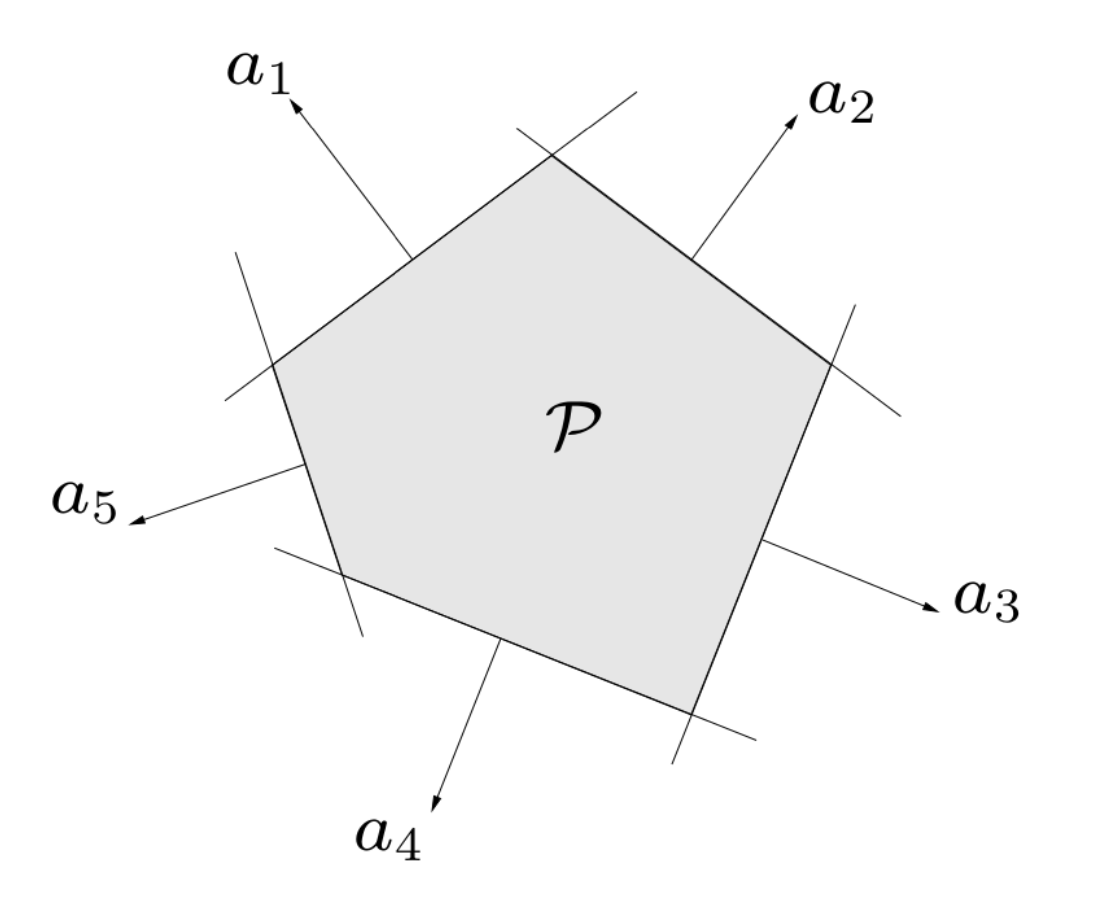
\includegraphics[width=.5\textwidth]{convex-problems/polyhedron.png}
        \caption{A polyhedron $\Pc$, the feasible set of a linear programming problem.}
    \end{figure}
\end{definition}

As an example, we consider the problem of finding the Chebyshev center of a polyhedron.
\begin{definition}[Chebyshev center]
    Given a polyhedron $\Pc$ of the form:
    \begin{equation*}
        \Pc = \set{x}{\forall i\in\iset{1}{m}, \: a_i^\tp x\leq b_i,}
    \end{equation*}
    its \emph{Chebyshev center} is the center of the largest inscribed ball. Recall that the ball $B(x_c, r)$ of center $x_c$ and radius $r$ is defined as:
    \begin{equation*}
        B(x_c, r) = \set{x}{\norm{x-x_c}_2\leq r}
    \end{equation*}
    Then, the Chebyshev center $\hat{x}$ is the point $x_c$ that maximizes $r$:
    \begin{equation*}
        \hat{x} = \argmin_{x_c, r} \set{r\in\R_+}{B(x_c, r)\subseteq\Pc} = \argmin_{x_c} \max_{x\in\Pc} \norm{x-x_c}_2
    \end{equation*}
\end{definition}

\begin{property}[Chebyshev center as a linear programming problem]
    The Chebyshev center of a polyhedron $\Pc$ can be computed as the solution of the following linear programming problem:
    \begin{equation*}
        \text{maximize } r \quad\text{subject to}\quad \forall i\in\iset{1}{m}, \: a_i^\tp x_c + r\norm{a_i}_2\leq b_i
    \end{equation*}
\end{property}

\subsubsection{Convex quadratic programming (QP)}
\begin{definition}[Quadratic programming problem]
    A \emph{quadratic programming} (QP) problem is an optimization problem in which the objective function is quadratic and the constraints are linear:
    \begin{equation*}
        \text{minimize } \frac{1}{2}x^\tp P x + q^\tp x + r\quad\text{subject to}\: \begin{cases}
            Gx\leq h\\
            Ax=b
        \end{cases}
    \end{equation*}
    where $P\in\Sb_n^+(\R)$ is positive semidefinite.

    The feasible set of a quadratic programming problem is a still polyhedron $\Pc$ (since the constraints have the same form as an LP problem). Solving a QP problem corresponds to minimizing a quadratic function over a polyhedron.

    \begin{figure}[H]
        \centering
        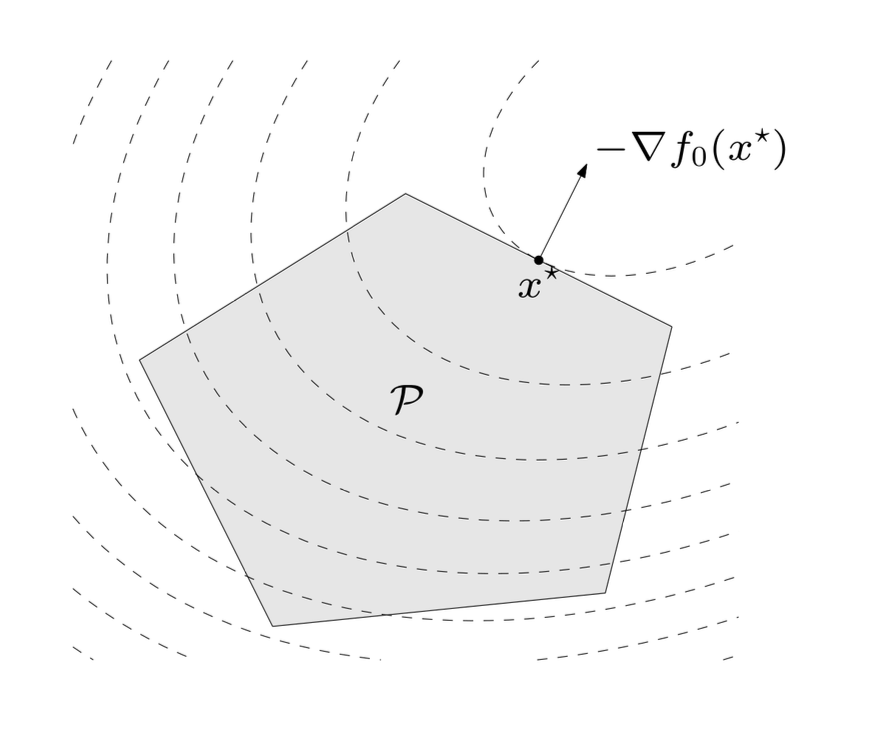
\includegraphics[width=.5\textwidth]{convex-problems/quadratic.png}
        \caption{A quadratic function over a polyhedron.}
    \end{figure}
\end{definition}

\begin{example}[Least squares problem]
    The least squares problem can be written as a QP problem:
    \begin{equation*}
        \text{minimize } \norm{Ax-b}_2^2
    \end{equation*}
    The analytical solution can be expressed using the Moore-Penrose pseudo-inverse of $A$, $A^\dagger$:
    \begin{equation*}
        x^* = A^\dagger b = (A^\tp A)^{-1}A^\tp b
    \end{equation*}
    Linear constraints such as $I\leq x\leq u$ can be added. 

    Another common variant is the LASSO regularization:
    \begin{equation*}
        \text{minimize } \norm{Ax-b}_2^2 + \lambda\norm{x}_1
    \end{equation*}
\end{example}

\begin{example}[Linear program with random cost]
    Consider a random vector $c\in\R^n$ with mean $\E[c] =: \bar{c}$ and covariance matrix $\V(c) =: \Sigma$. The following linear program is often used in economics and finance:
    \begin{equation*}
        \text{minimize } \E[c^\tp x] + \gamma\V(c^\tp x) = \bar{c}^\tp x + \gamma x^\tp\Sigma x \quad\text{subject to}\quad \begin{cases}
            Gx\leq h\\
            Ax=b
        \end{cases}
    \end{equation*}
    Where $\gamma>0$ is a risk-aversion parameter: it controls how much we penalize the variance of the cost. Higher values of $\gamma$ allow for solutions with higher expected cost but lower variance.
\end{example}

\subsubsection{Quadratically constrained quadratic programming (QCQP)}
\begin{definition}[Quadratically constrained quadratic programming problem]
    A \emph{quadratically constrained quadratic programming} (QCQP) problem is an optimization problem in which both the objective function and the constraints are quadratic:
    \begin{equation*}
        \text{minimize } \frac{1}{2}x^\tp P_0 x + q_0^\tp x + r_0\quad\text{subject to}\: \begin{cases}
            \frac{1}{2}x^\tp P_i x + q_i^\tp x + r_i\leq0, \quad\forall i\in\iset{1}{m}\\
            Ax=b
        \end{cases}
    \end{equation*}
    where the objective and constraints matrices $P_i\in\Sb_n^+(\R)$ are positive semidefinite. In the case where $P_1, \dots, P_m\in\Sb_n^{++}(\R)$ are positive definite, the feasible region is the intersection of $m$ ellipsoids and an affine set.
\end{definition}

\subsubsection{Second-order cone programming (SOCP)}
\begin{definition}[Second-order cone programming problem]
    A \emph{second-order cone programming} (SOCP) problem is an optimization problem in which the objective function is linear, and the constraints are second-order cones:
    \begin{equation*}
        \text{minimize } f^\tp x \quad\text{subject to}\: \begin{cases}
            \norm{A_i x + b_i}_2\leq c_i^\tp x + d_i, \quad\forall i\in\iset{1}{m}\\
            Fx=g
        \end{cases}
    \end{equation*}
    where $f\in\R^n$, $A_i\in\mathscr{M}_{n_i, n}(\R)$, $b_i\in\R^{n_i}$, $c_i\in\R^{n_i}$, $d_i\in\R$, $F\in\mathscr{M}_{p, n}(\R)$, $g\in\R^p$.

    Inequalities are second-order cone (SOC) constraints:
    \begin{equation*}
        (A_ix+b_i, c_i^\tp x+d_i)\in \text{second-order cone in } \R^{n_i+1}
    \end{equation*}
    For $n_i=0$, this reduces to an LP problem. If $c_i=0$, this reduces to a QCQP problem. In general, SOCP problems are more general than LP and QCQP problems.
\end{definition}

\subsection{Robust linear programming}
\subsubsection{Introduction}
In many situations, the parameters of an optimization problems might be uncertain. For instance, in an LP problem such as:
\begin{equation*}
    \text{minimize } c^\tp x \quad\text{subject to}\quad \forall i\in\iset{1}{m}, \: a_i^\tp x\leq b_i
\end{equation*}
there can be uncertainty on the values of $c, a_i, b_i$, which can be modeled as taking any value in given intervals. There are two common approaches to handle this uncertainty: deterministic and stochastic models. Assume that the value of $a_i$ can be any value in the set $\Ec_i$.

A \textbf{deterministic model} solves a harder problem, in which the constraints must hold for all $a_i\in\Ec_i$. This can be written as:
\begin{equation*}
    \text{minimize } c^\tp x \quad\text{subject to}\quad \forall i\in\iset{1}{m}, \: \underbrace{\forall a_i\in\Ec_i}_{\text{uncertainty}}, \: a_i^\tp x\leq b_i
\end{equation*}

A \textbf{stochastic model} uses chance constraints: we consider that $a_i$ is a random variable, and we require that the constraints hold with a given probability $\eta$. This can be written as:
\begin{equation*}
    \text{minimize } c^\tp x \quad\text{subject to}\quad \forall i\in\iset{1}{m}, \: \underbrace{\P(a_i^\tp x\leq b_i)\geq\eta}_{\text{probability constraint}}
\end{equation*}

In the following, we will develop both approaches using SOCP.

\subsubsection{Deterministic approach via SOCP}
We can model the uncertainty on $a_i$ by choosing an ellipsoid as $\Ec_i$:
\begin{equation*}
    \Ec_i = \set{\bar{a}_i+P_iu}{\norm{u}_2\leq1}
\end{equation*}
where $\bar{a}_i\in\R^n$ are the centers, and the semi-axes are determined by the singular values and vectors of $P_i\in\mathscr{M}_n(\R)$. Therefore, the robust LP problem of the form:
\begin{equation*}
    \text{minimize } c^\tp x \quad\text{subject to}\quad \forall i\in\iset{1}{m}, \: \forall a_i\in\Ec_i, \: a_i^\tp x\leq b_i
\end{equation*}
can be written as the following SOCP problem:
\begin{equation*}
    \text{minimize } c^\tp x \quad\text{subject to}\quad \forall i\in\iset{1}{m}, \: \bar{a}_i^\tp x + \norm{P_i^\tp x}_2\leq b_i
\end{equation*}
This comes from the fact that:
\begin{equation*}
    \sup_{\norm{u}_2\leq1} (\bar{a}_i + P_iu)^\tp x = \bar{a}_i^\tp x + \norm{P_i^\tp x}_2
\end{equation*}
hence, if $\bar{a}_i^\tp x + \norm{P_i^\tp x}_2\leq b_i$ holds, then $a_i^\tp x\leq b_i$ holds for all $a_i\in\Ec_i$.

\subsubsection{Stochastic approach via SOCP}
Assume that $a_i$ is Gaussian with mean $\bar{a}_i$ and covariance matrix $\Sigma_i$:
\begin{equation*}
    a_i\sim\Nc(\bar{a}_i, \Sigma_i)
\end{equation*}
Therefore, $a_i^\tp x$ is a Gaussian random vector with mean $\bar{a}_i^\tp x$ and variance $x^\tp\Sigma_i x$. We can model the probability constraint as:
\begin{equation*}
    \P(a_i^\tp x\leq b_i)=\Phi\left(\frac{b_i-\bar{a}_i^\tp x}{\norm{\Sigma_i^{1/2}x}_2}\right)
\end{equation*}
where $\Phi(x)=(1/\sqrt{2\pi})\int_{-\infty}^x e^{-t^2/2}dt$ is the \emph{Cumulative Distribution Function} (CDF) of $\Nc(0,1)$. The robust LP problem can be written as:
\begin{equation*}
    \text{minimize } c^\tp x \quad\text{subject to}\quad \forall i\in\iset{1}{m}, \: \P(a_i^\tp x\leq b_i)\geq\eta
\end{equation*}
This can be written as the following SOCP problem:
\begin{equation*}
    \text{minimize } c^\tp x \quad\text{subject to}\quad \forall i\in\iset{1}{m}, \: \bar{a}_i^\tp x+\Phi^{-1}(\eta)\norm{\Sigma_i^{1/2}x}_2\leq b_i
\end{equation*}
which is an SOCP problem when $\Phi^{-1}(\eta)\geq0$, verified for $\eta\geq1/2$. For values of $\eta<1/2$, the problem is non-convex, as can be seen in the following visualization.
\begin{figure}[H]
    \centering
    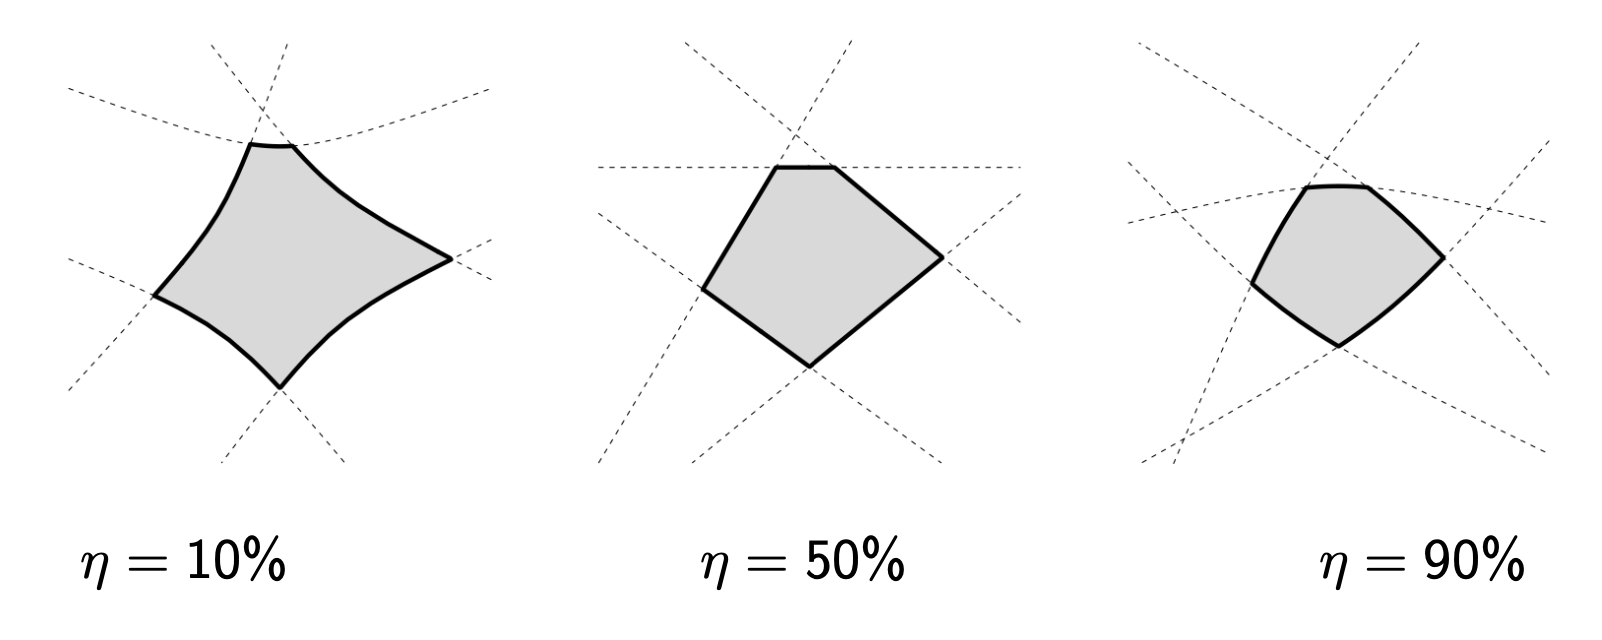
\includegraphics[width=.8\textwidth]{convex-problems/reliability.png}
    \caption{The set $\set{x}{\forall i\in\iset{1}{m}, \: \P(a_i^\tp x\leq b_i)\geq\eta}$ for multiple values of $\eta$. It is convex for $\eta\geq1/2$ and in general non-convex for $\eta<1/2$.}
\end{figure}

\subsection{Generalized inequalities}
For multiple reasons, it can be useful to consider more general inequalities than the standard ones, in the sense that the inequalities are not necessarily defined on the real line. This is mainly motivated by semi-definite programming, where the inequalities must hold on the cone of positive semidefinite matrices. We first define a partial ordering $\succcurlyeq$ on a cone $K$, and use it to introduce generalized inequalities.

\subsubsection{Convex cone properties}
Recall that a set $K$ is a convex cone if:
\begin{equation*}
    x_1, x_1\in K \implies \forall\theta_1, \theta_2>0, \quad \theta_1x_1+\theta_2x_2\in K
\end{equation*}

\begin{definition}
    A convex cone $K$ can have the following properties:
    \begin{itemize}
        \item \emph{pointed}: if it contains $0$
        \item \emph{salient}: if it contains no line, that is $x\in K \land -x\in K\implies x=0$
        \item \emph{solid}: if it has a non-empty interior ($\mathring{K}\neq\emptyset$)
        \item \emph{closed}: if $K^\subset$ is an open set
    \end{itemize}
\end{definition}

\begin{definition}[Notation]
    Let $K$ be a pointed, salient and solid convex cone. Let $A$ and $B$ be two points of the ambient space.
    \begin{itemize}
        \item We note $A\succcurlyeq_K 0$ if and only if $A\in K$.
        \item We note $A\succcurlyeq_K B$ if and only if $A-B\succcurlyeq_K 0$.
        \item We note $A\succ_K 0$ if and only if $A\in\mathring{K}$ (which makes sense if $K$ is solid).
    \end{itemize}
    \begin{figure}[H]
        \centering
        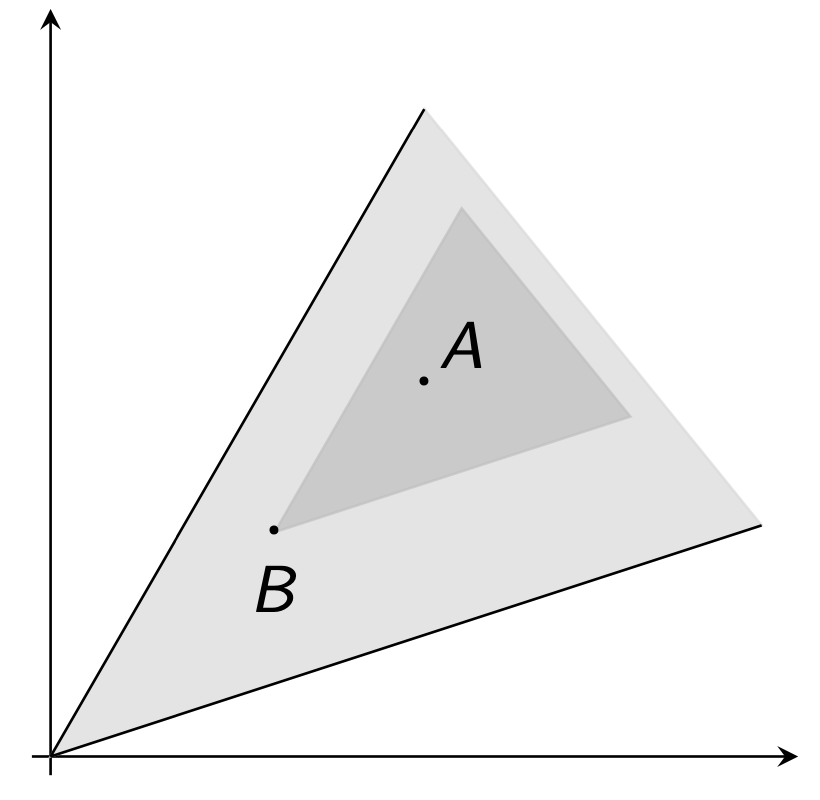
\includegraphics[width=.3\textwidth]{convex-problems/cone.png}
    \end{figure}
\end{definition}

\begin{property}
    $\succcurlyeq_K$ defines a partial ordering.
\end{property}
\begin{proof}$ $
    \begin{itemize}
        \item $K$ is pointed, hence $0\in K$, hence for any $A$ we have that $A-A\succcurlyeq_K 0$ and $A\succcurlyeq_K A$.
        \item $A\succcurlyeq_K B$ and $B\succcurlyeq_K A$ implies that $A-B\in K$ and $B-A\in K$. Since $K$ is salient, $A-B=0$ and $A=B$.
        \item $A\succcurlyeq_K B$ and $B\succcurlyeq_K C$ implies that $A-B\in K$ and $B-C\in K$. Therefore, $A-C=(A-B)+(B-C)\in K$ since $K$ is a cone, and therefore $A\succcurlyeq_K C$.
    \end{itemize}
\end{proof}

\begin{definition}[Convex problem with generalized inequality constraints]
    A \emph{convex optimization problem with generalized inequality} constraints is a problem of the form:
    \begin{equation*}
        \text{minimize } f(x) \quad\text{subject to}\quad \begin{cases}
            \forall i\in\iset{1}{m}, \: g_i(x)\preccurlyeq_{K_i} 0\\
            Ax=b
        \end{cases}
    \end{equation*}
    where $f:\R^n\to\R$ is convex, and the $g_i:\R^n\to\R^{k_i}$ are $K_i$-convex with respect to the proper cones $K_i$:
    \begin{equation*}
        \forall i\in\iset{1}{m}, \: \forall x, y\in\R^n, \: \forall\theta\in[0,1], \quad g_i(\theta x+(1-\theta)y)\preccurlyeq_{K_i} \theta g_i(x)+(1-\theta)g_i(y)
    \end{equation*}
\end{definition}
A convex optimization problem with generalized inequality constraints as the same properties as a standard convex problem: its feasible set is convex, any local optimum is a global optimum, etc. When the $K_i$ are clear from the context, we can simply use $\preccurlyeq$ and omit the $K_i$.

\begin{definition}[Conic convex optimization problem]
    A \emph{conic convex optimization problem} is a special case of the generalized convex problem, where the objective and the constraints are affine:
    \begin{equation*}
        \text{minimize } c^\tp x \quad\text{subject to}\quad \begin{cases}
            Fx+g\preccurlyeq_K 0\\
            Ax=b
        \end{cases}
    \end{equation*}
    where $c\in\R^n$, $F\in\mathscr{M}_{p, n}(\R)$, $g\in\R^p$, $A\in\mathscr{M}_{m, n}(\R)$. This extends linear programming to non-polyedral cones. The linear programming case can be obtained by choosing $K=\R_+^m$.
\end{definition}

\subsubsection{Semidefinite programming (SDP)}
\begin{definition}
    A \emph{semidefinite programming} (SDP) problem is a problem of the form:
    \begin{equation*}
        \text{minimize } c^\tp x \quad\text{subject to}\quad \begin{cases}
            x_1G_1+\dots+x_nG_n+H\preccurlyeq 0\\
            Ax=b
        \end{cases}
    \end{equation*}
    where $G_i, H\in\Sb_k(\R)$. 
    
    \begin{remark}
        The inequality constraint is called a \emph{linear matrix inequality} (LMI). Note that problems with multiple LMIT constraints can be transformed into a single LMI constraint of higher dimension. Suppose that you have the constraints:
        \begin{equation*}
            x_1\hat{G}_1+\dots+x_n\hat{G}_n+\hat{H}\preccurlyeq0 \quad\text{and}\quad x_1\tilde{G}_1+\dots+x_n\tilde{G}_n+\tilde{H}\preccurlyeq0
        \end{equation*}
        They can be rewritten as a single LMI:
        \begin{equation*}
            x_1\begin{bmatrix}
                \hat{G}_1 & 0\\
                0 & \tilde{G}_1
            \end{bmatrix}
            +\dots+
            x_n\begin{bmatrix}
                \hat{G}_n & 0\\
                0 & \tilde{G}_n
            \end{bmatrix}
            +\begin{bmatrix}
                \hat{H} & 0\\
                0 & \tilde{H}
            \end{bmatrix}\preccurlyeq0
        \end{equation*}
    \end{remark}
\end{definition}

\begin{example}[Largest eigenvalue minimization]
    Consider the following problem:
    \begin{equation*}
        \text{minimize } \lambda_{\max}(A(x))
    \end{equation*}
    where $A(x)=A_0+x_1A_x+\dots+x_nA_n$ and $A_0, A_1, \dots, A_n\in\Sb_k(\R)$. This problem can be written as an equivalent SDP problem:
    \begin{equation*}
        \text{minimize } t \quad\text{subject to}\quad A(x)\preccurlyeq tI
    \end{equation*}
    over variables $x\in\R^n$ and $t\in\R$. This follows from:
    \begin{equation*}
        \lambda_{\max}(A(x))\leq t \iff A(x)\preccurlyeq tI
    \end{equation*}
\end{example}

\begin{example}[Matrix norm minimization]
    Consider the following problem:
    \begin{equation*}
        \text{minimize } \norm{A(x)}_2 = \sqrt{\lambda_{\max}(A(x)^\tp A(x))}
    \end{equation*}
    where $A(x)=A_0+x_1A_x+\dots+x_nA_n$ and $A_i\in\Sb_k(\R)$. This problem can be written as an equivalent SDP problem:
    \begin{equation*}
        \text{minimize } t \quad\text{subject to}\quad \begin{bmatrix}
            tI & A(x)\\
            A(x)^\tp & tI
        \end{bmatrix}\succeq0
    \end{equation*}
    over variables $x\in\R^n$ and $t\in\R_+$. This follows from:
    \begin{equation*}
        \norm{A(x)}_2\leq t \iff A^\tp A\preccurlyeq t^2I \iff \begin{bmatrix}
            tI & A(x)\\
            A(x)^\tp & tI
        \end{bmatrix}\succeq0
    \end{equation*}
    where the last equivalence comes from the Schur complement.
\end{example}

\subsubsection{LPs and SOCPs as SDPs}
\begin{property}[Any LP problem is equivalent to an SDP problem]
    Consider the LP problem:
    \begin{equation*}
        \text{minimize } c^\tp x \quad\text{subject to}\quad Ax\leq b
    \end{equation*}
    This can be written as the following SDP problem:
    \begin{equation*}
        \text{minimize } c^\tp x \quad\text{subject to}\quad \diag(Ax-b)\preccurlyeq0
    \end{equation*}
\end{property}

\begin{property}[Any SOCP problem is equivalent to an SDP problem]
    Consider the SOCP problem:
    \begin{equation*}
        \text{minimize } f^\tp x \quad\text{subject to}\quad \forall i\in\iset{1}{m}, \: \norm{A_ix+b_i}_2\leq c_i^\tp x+d_i
    \end{equation*}
    This can be written as the following SDP problem:
    \begin{equation*}
        \text{minimize } f^\tp x \quad\text{subject to}\quad \forall i\in\iset{1}{m}, \: \begin{bmatrix}
            c_i^\tp x+d_i & A_ix+b_i\\
            (A_ix+b_i)^\tp & c_i^\tp x+d_i
        \end{bmatrix}\succcurlyeq0
    \end{equation*}
\end{property}

\subsection{Quasi-convex problems}
\subsubsection{Quasi-convex functions}
\begin{definition}[Quasi-convex function]
    A function $f:\R^n\to\R$ is \emph{quasi-convex} if $\dom f$ is convex at the sublevel sets; that is, for all $\alpha\in\R$, the set $S_\alpha$ is convex:
    \begin{equation*}
        S_\alpha := \set{x\in\dom f}{f(x)\leq\alpha}
    \end{equation*}
    \begin{figure}[H]
        \centering
        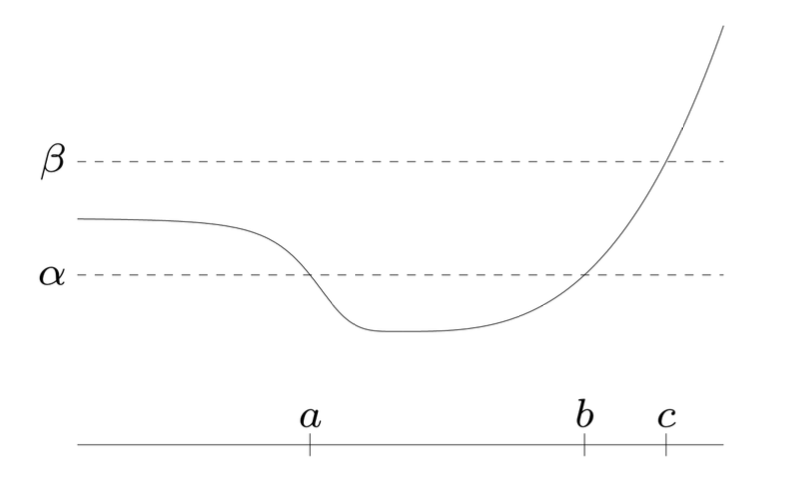
\includegraphics[width=.5\textwidth]{convex-problems/quasiconvex.png}
        \caption{A quasi-convex function.}
    \end{figure}
\end{definition}

\begin{definition}[Quasi-concave function]
    A function $f$ is \emph{quasi-concave} if $-f$ is quasi-convex.
\end{definition}

\begin{definition}[Quasi-linear function]
    A function $f$ is \emph{quasi-linear} if it is both quasi-convex and quasi-concave.    
\end{definition}

\begin{example}$ $
    \begin{itemize}
        \item $x\mapsto \sqrt{|x|}$ is quasi-convex on $\R$
        \item $x\mapsto \lfloor x\rfloor$ is quasi-linear
        \item $\log x$ is quasi-linear on $\R_+^*$
        \item $f(x_1, x_2) = x_1x_2$ is quasi-concave on $(\R_+^*)^2$
        \item Any linear-fractional function is quasi-linear:
        \begin{equation*}
            f(x)=\frac{a^\tp x+b}{c^\tp x+d}
        \end{equation*}
        where $\dom f = \set{x}{c^\tp x+d>0}$
        \item The distance ratio is quasi-convex:
        \begin{equation*}
            f(x) = \frac{\norm{x-a}_2}{\norm{x-b}_2}
        \end{equation*}
        where $\dom f = \set{x}{\norm{x-a}_2\leq\norm{x-b}_2}$.
    \end{itemize}
\end{example}

\begin{property}[Modified Jensen inequality]
    Let $f$ be a quasi-convex function, and $x, y\in\dom f$. Then, for all $\theta\in[0,1]$:
    \begin{equation*}
        f(\theta x+(1-\theta)y)\leq\max(f(x), f(y))
    \end{equation*}
\end{property}

\begin{property}[First-order condition]
    A differentiable function $f$ with convex domain is quasi-convex if and only if:
    \begin{equation*}
        \forall x\in\dom f, \: \forall y\in\dom f, \: f(y)\leq f(x) \implies \nabla f(x)^\tp (y-x)\leq 0
    \end{equation*}
    \begin{figure}[H]
        \centering
        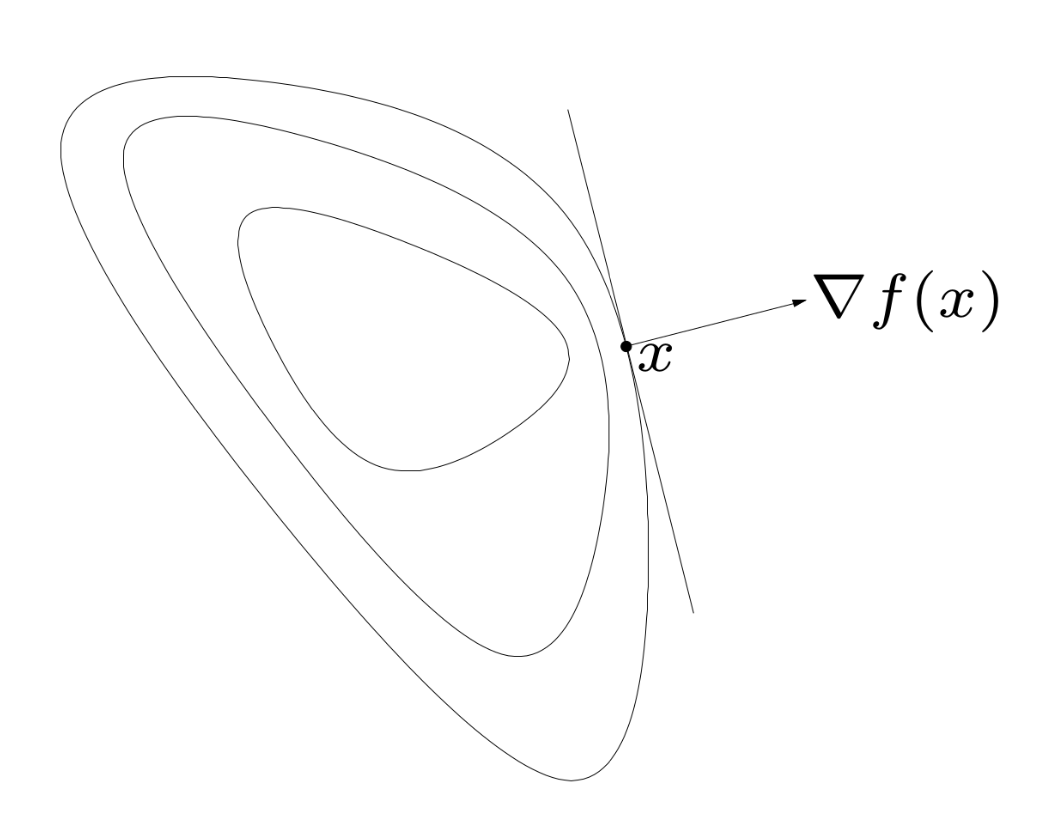
\includegraphics[width=.35\textwidth]{convex-problems/fo-condition.png}
    \end{figure}
\end{property}

\begin{remark}
    The sum of two quasi-convex functions is not necessarily quasi-convex.
\end{remark}

\subsubsection{Quasi-convex optimization}
\begin{definition}[Quasi-convex optimization problem]
    A \emph{quasi-convex optimization problem in standard form} is an optimization problem in which the objective function is quasi-convex and the constraints are convex:
    \begin{equation*}
        \text{minimize } f(x) \quad\text{subject to}\quad \begin{cases}
            \forall i\in\iset{1}{m}, \: g_i(x)\leq 0\\
            \forall i\in\iset{1}{m}, \: a_i^\tp x = b_i
        \end{cases}
    \end{equation*}
    where $f$ is \textbf{quasi-convex}, and the $g_i$ are convex.
\end{definition}

\begin{remark}
    Such a problem can have locally optimal points that are not globally optimal.
    \begin{figure}[H]
        \centering
        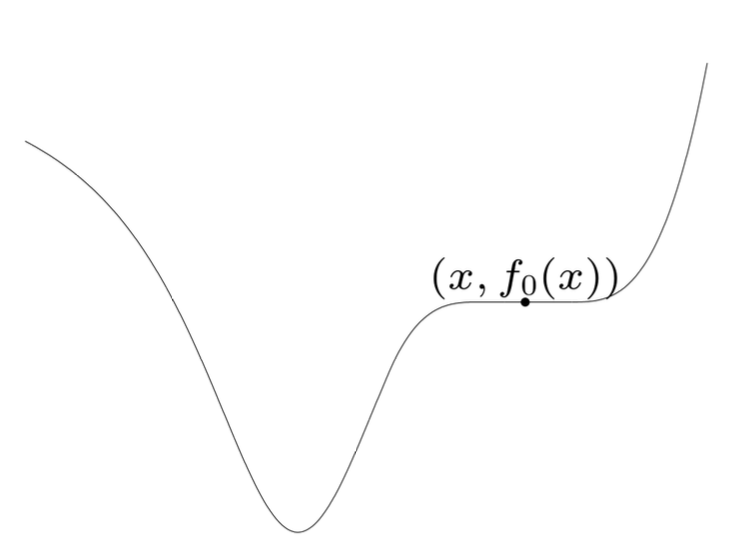
\includegraphics[width=.4\textwidth]{convex-problems/non-global.png}
    \end{figure}
\end{remark}

\subsubsection{Quasi-convex optimization via bisection}
Consider for a fixed $t$ consider the following feasibility problem in $x$:
\begin{equation}
    \label{eq:quasi-convex-feasibility}
    \text{find } x \quad\text{subject to}\quad \begin{cases}
        f(x)\leq t\\
        \forall i\in\iset{1}{m}, \: g_i(x)\leq 0\\
        Ax=b
    \end{cases}
\end{equation}
where $f$ is quasi-convex and the $g_i$ are convex.

If this problem is feasible, we can conclude that $t\geq p^*$; if it is infeasible, $t\leq p^*$. This leads to the following bisection algorithm, acting as a binary search. Consider two initial values $I_0<u_0$. We simply repeat the following steps:
\begin{enumerate}
    \item $t:=(I+u)/2$
    \item Solve the convex feasibility problem \eqref{eq:quasi-convex-feasibility}
    \item If \eqref{eq:quasi-convex-feasibility} is feasible, $u:=t$; otherwise, $I=t$.
\end{enumerate}
This requires $\lceil \log_2((u_0-I_0)/\epsilon)\rceil$ iterations to obtain an optimality gap of at most $\epsilon$.

\subsection{Examples}
We present two common applications in statistical learning, taking the form of optimization problems: regression and classification.
\subsubsection{Regression}
Consider a set of data formed of vectors $x_i\in\R^d$ and labels $y_i\in\R$:
\begin{equation*}
    \set{(x_i, y_i)}{i\in\iset{1}{n}} \subset \R^d\times\R
\end{equation*}
We can form the following data matrix $X$ and labels vector $Y$:
\begin{equation*}
    X:=\begin{bmatrix}x_1 & x_2 & \cdots & x_n\end{bmatrix}
    \quad\text{and}\quad
    Y:=\begin{bmatrix}y_1 \\ y_2 \\ \vdots \\ y_n\end{bmatrix}
\end{equation*}
The goal of linear regression is to find a $\theta\in\R^d$ such that:
\begin{equation*}
    X^\tp\theta \simeq Y
\end{equation*}
This can be done by solving the \emph{Least Absolute Shrinkage and Selection Operator} (LASSO) of parameter $\lambda>0$:
\begin{equation*}
    \min_\theta \norm{X^\tp\theta-Y}_2^2 + \lambda\norm{\theta}_1
\end{equation*}

\subsubsection{Classification}
Consider a set of data formed of vectors $x_i\in\R^d$ and labels $y_i\in\{-1, 1\}$:
\begin{equation*}
    \set{(x_i, y_i)}{i\in\iset{1}{n}} \subset \R^d\times\{-1, 1\}
\end{equation*}

The hard-margin \emph{Support Vector Machine} (SVM) is defined as:
\begin{equation*}
    \text{find } w\in\R^d \quad\text{such that}\quad \forall i\in\iset{1}{n}, \: y_i(w^\tp x_i+b)\geq 1
\end{equation*}
This problem can be solved via optimization by maximizing the margin $2/\norm{w}_2$:
\begin{equation*}
    \minimize_w \norm{w}_2^2 \quad\text{such that}\quad \forall i\in\iset{1}{n}, \: y_i(w^\tp x_i+b)\geq 1
\end{equation*}
The soft-margin SVM is defined as:
\begin{equation*}
    \minimize_{s\geq0, w} \lambda\norm{w}_2^2 + \sum_{i=1}^n s_i \quad\text{such that}\quad \forall i\in\iset{1}{n}, \: y_i(w^\tp x_i+b)\geq 1
\end{equation*}